\documentclass[12pt]{article}
\usepackage{fullpage,enumitem,amsmath,amssymb,graphicx}
\usepackage{graphicx} % This is a package for including graphics in your solution.
\usepackage{listings}
\usepackage[final]{pdfpages}

\begin{document}

\begin{center}
{\Large CS168 Spring Assignment 7}

\begin{tabular}{rl}
SUNet ID(s): 05794739 & \\
Name(s): & Luis A. Perez \\
Collaborators: &
\end{tabular}
\end{center}

By turning in this assignment, I agree by the Stanford honor code and declare
that all of this is my own work.

\section*{Part 1}

\begin{enumerate}[label=(\alph*)]
  \item
    \begin{enumerate}
      \item The circle graph with $n=10$ is periodic and irreducible.

      This is because it is bipartite. Consider partitions $A,B$ where even nodes are in $A$ and odd nodes in $B$. Then the edges $(u,v)$ exists only if $u \in A, v \in B$. As such, it has a period of $2$.

      It is irreducible because one can reach any state from any other state.
      \item The circle graph with $n=9$ is aperiodic and irreducible.

      Consider any pair of distinct nodes $i,j$. WLOG, suppose $i < j$. Then we can reach $j$ from $i$ in $j-i$ steps as well as $9 - (j-i)$. Note that $j - i \in \{1, 2, 3, 4, 5, 6, 7, 8\}$ and, correspondingly, we'd have $9 - (j-i) \in \{8, 7, 6, 5, 4, 3, 2, 1\}$. The only pairs for which the GCD is not $1$ are $(3, 6), (6,3)$. However, if we can reach a node in $3$ steps, we can reach it in $5$ (just go back once and foward again). As such, even for these nodes, the GCD for times at which they are reachable is $1$.

      It is irreducible because one can reach any state from any other state.

      The stationary distribution $\pi$ is the uniform distribution over all states. To see why, note that all states are symmetric and interchangeable, so the stationary distribution must be uniform. There are $9$ states, so we have:
      \[
        \pi_i = \frac{1}{9} \text{ for all } 1 \leq i \leq 9
      \]
      \item The circle graph with $n=9$ and an extra edges connecting nodes $1$ and $5$ is aperiodic and irreducible.

      Ignoring the extra edge, we already know it's aperiodic as per (2). As such, we only need to verify that the states $1$ and $5$ are still aperiodic. They are, since we can reach them in either $4$ steps or $5$ steps.   

      It is irreducible because one can reach any state from any other state.

      The stationary distribution $\pi$ is no longer uniform. However, we can compute it easily. We have $7$ nodes with two edges, and two nodes with $3$. As such, we have $2*7 + 3*2 = 20$ distributions. As such, we have:
      \[
        \pi_i = \frac{1}{10} \quad i \neq 1,5
        \pi_i = \frac{3}{20} \quad i = 1, 5
      \]
    \end{enumerate}
  \item We plot the variational distance from the distribution at time $t$ to the stationary distribution (we use the inform distribution for graphs which are either periodic or reducible). For the results, see Figure \ref{fig:mixing_time}.

  \begin{figure}[!ht]
    \centering
    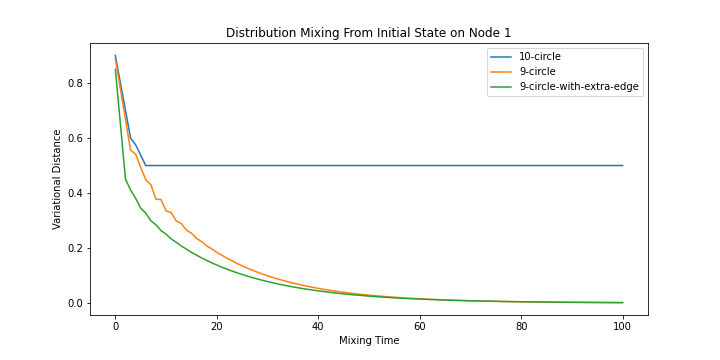
\includegraphics[scale=0.5]{figures/mixing_time.png}
    \caption{Plot of variational distance between true distribution at time $t$ and stationary distribution for each of the discussed graphs. If no stationary distribution exists (eg, for the $10$ node circle graph), we use the uniform distribution.}
    \label{fig:mixing_time}
  \end{figure}

  The code used to generate the above is here:
  \begin{verbatim}
def circle_graph(n=10):
    """Returns transition matrix for a circle graph."""
    A = np.zeros((n, n))
    for i in range(n):
        A[i, (i + 1) % n] = 1
        A[(i + 1) % n, i] = 1
    return 0.5 * A, 1 / n * np.ones((1, n))

def circle_graph_with_extra_edge(n=10, a=1, b=5):
    """Same as above but for a circle graph with an additional edge (a,b)."""
    P, _ = circle_graph(n=n)
    P[a-1, b-1] = 0.5
    P[b-1, a-1] = 0.5
    P[a-1, :] = P[a-1, :] * 2 / 3
    P[b-1, :] = P[b-1, :] * 2 / 3
    denom = 2*(n-2) + 3*2
    pi = 2 * np.ones((1, n)) / denom
    pi[0, a - 1] = 3 / denom
    pi[0, b - 1] = 3 / denom
    
    return P, pi

def variation_distance(x, y):
    return 1 / 2 * np.sum(np.abs(x - y))

def chain_mixing(T, pi):
    s = np.zeros((1, np.shape(T)[0]))
    s[0, 0] = 1
    distance = [variation_distance(s, pi)]
    for t in range(1, 101):
        s = np.dot(s, T)
        distance.append(variation_distance(s, pi))
        
    return distance

def problem1b():
    graphs = {
        '10-circle' : circle_graph(n=10),
        '9-circle': circle_graph(n=9),
        '9-circle-with-extra-edge': circle_graph_with_extra_edge(n=9)
    }
    for name, (T, pi) in graphs.items():
        dists = chain_mixing(T, pi)
        plt.plot(range(len(dists)), dists, label=name)
    plt.legend()
    plt.title('Distribution Mixing From Initial State on Node 1')
    plt.ylabel('Variational Distance')
    plt.xlabel('Mixing Time')
    plt.savefig('figures/mixing_time.png', format='png')
    plt.close()

problem1b()
  \end{verbatim}
  
  \item
    10-circle has $\lambda_2=0.8090169943749482$.

    9-circle has $\lambda_2=0.766044443118978$.

    9-circle-with-extra-edge has $\lambda_2=0.7675918792439985$.

  \item
     While normally we'd expect a smaller $\lambda_2$ to indicates a faster convergence rate, for our specific initial state we see from the above that the $9$-graph with an extra edge actually has the faster convergence (despite a slightly larger second largest eigenvalue). The reason for this relates to the power iteration algorithm. We know that the ratio of the second largest eigenvector to the largest eigenvector determines the converged. In the case of a transtion matrix, this ratio entirely depends on the second largest eigenvector (the largest eigenvector is always $1$). So as this value is smaller, we'd expect fewer iteration. 

     However, this is a lose upperbound, and as we can see from our results above, it does not always hold. 
\end{enumerate}

\newpage
\section*{Part 2}

\begin{enumerate}[label=(\alph*)]
  \item Each state corresponds to a unique permutation of the parks we visit. As such, there are a total of $30!$ states, which is an extremely large number of possible states.

  For the casee where $T = 0$, we will not see all possible routes no matter how large MAXITER is. The reason for this is that we will be doing only a local search. Note that for a given route, there are only $n$ possible transitions out of that route. If our current route is a local minimum amongst these, we'll never escape.

  On the other hand, when $T > 0$, we will eventually see all possible routes. The reason is that there is a non-zero probability of taking, essentially, a random move. As such, there's a non-zero probability that we reach any state.

  The code implementing the algorithm is presented below:
  \begin{verbatim}
def mcmc(D, n_iters, T, route_fn):
    """Implements MCMC for Eucledian Traveling Salesmen on Distance Matrix D."""
    route = np.array(range(D.shape[0]))
    np.random.shuffle(route)
    best = route.copy()
    
    selected = np.random.choice(range(D.shape[0]), replace=True, size=n_iters)
    selected2 = np.random.choice(range(D.shape[0]), replace=True, size=n_iters)
    route_dists = []
    for idx, idx2 in zip(selected, selected2):
        newroute = route.copy()
        route_fn(route, newroute, idx, idx2)
        route_dist = route_length(D, route.tolist() + [route[0]])
        newroute_dist = route_length(D, newroute.tolist() + [newroute[0]])
        route_dists.append(route_dist)
        delta_dist = newroute_dist - route_dist
        if delta_dist < 0 or (T > 0 and np.random.uniform() < np.exp(-delta_dist / T)):
            route = newroute
        if route_length(D, route.tolist() + [route[0]]) < route_length(D, best.tolist() + [best[0]]):
            best = route
    return best, route_dists
  \end{verbatim}

  \item
    We try four values of $T \in \{0, 1, 10, 100\}$ in Figure \ref{fig:iteration_mcmc}. From the figure, we see that the value with $T = 10$ appears to perform the best. This also holds since over the ten trials, $T=10$ finds a tour of length $279.21$.

    \begin{figure}[!ht]
      \centering
      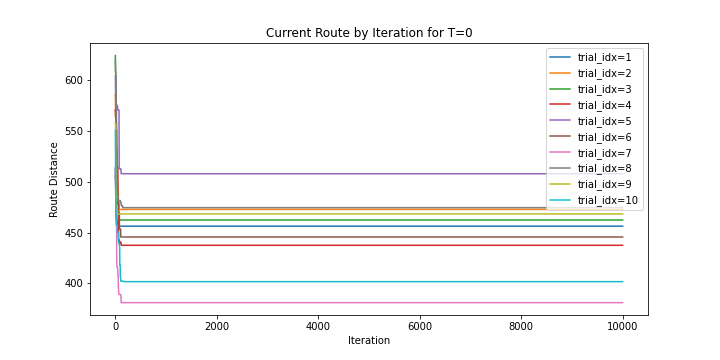
\includegraphics[scale=0.32]{figures/route_by_iteration_t=0.png}
      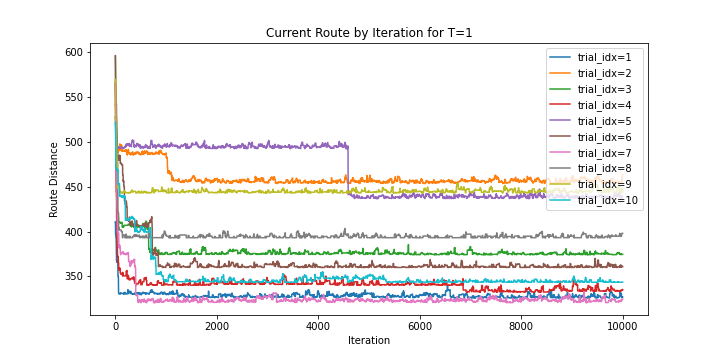
\includegraphics[scale=0.32]{figures/route_by_iteration_t=1.png}
      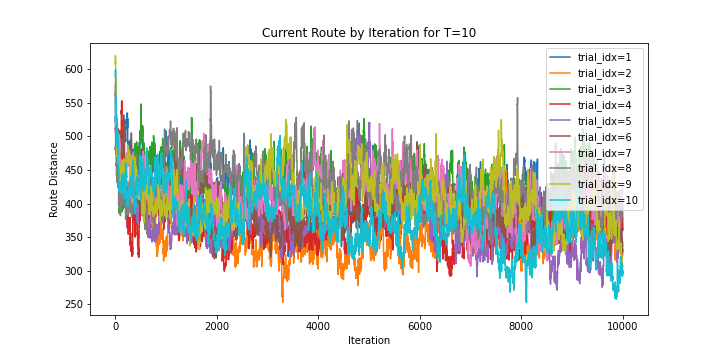
\includegraphics[scale=0.32]{figures/route_by_iteration_t=10.png}
      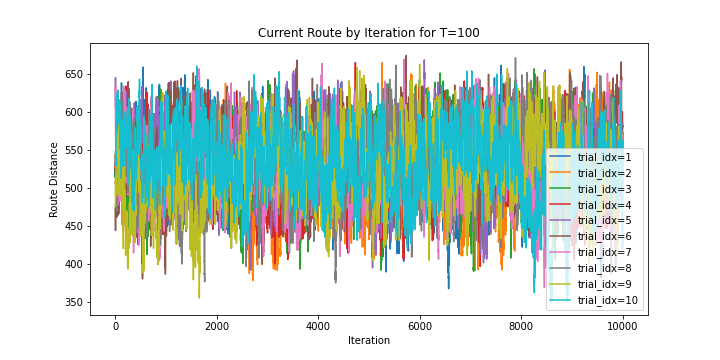
\includegraphics[scale=0.32]{figures/route_by_iteration_t=100.png}
      \caption{Searched Routes and Their Corresponding Tour Distance by Iteration for Different Temperature Values using Markov Chain Monte Carlo.}
      \label{fig:iteration_mcmc}
    \end{figure}

  \item
    We repeat the experiment with the new mechanism for choosing paths in Figure \ref{fig:iteration_mcmc_2}. It turns out that in this case, the best temperature parameter appears to be $T = 1$ which finds a tour length of $166.23$.

    \begin{figure}[!ht]
      \centering
      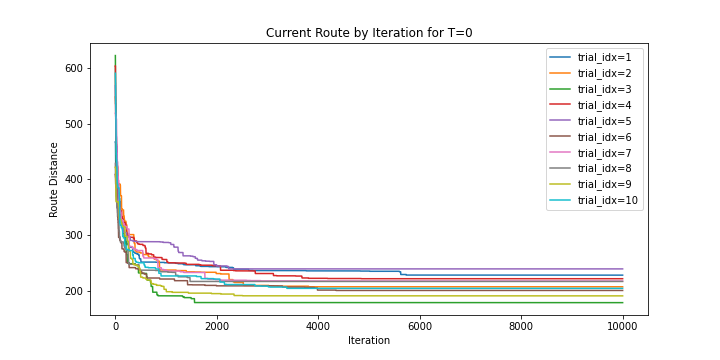
\includegraphics[scale=0.32]{figures/route_by_iteration_t=0_random.png}
      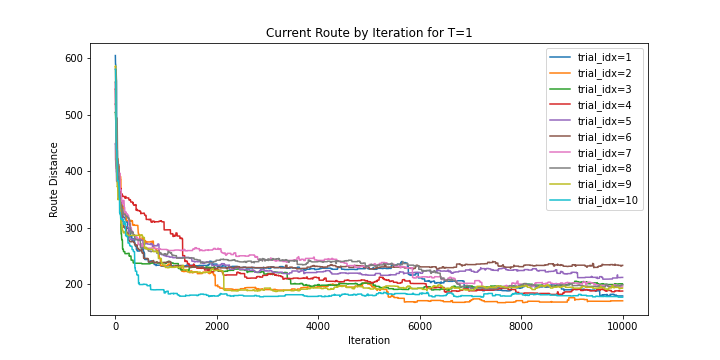
\includegraphics[scale=0.32]{figures/route_by_iteration_t=1_random.png}
      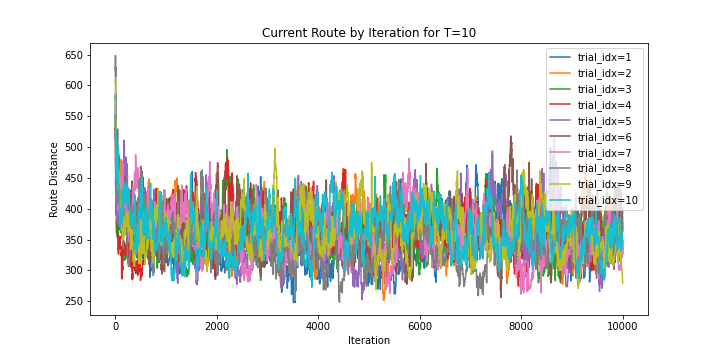
\includegraphics[scale=0.32]{figures/route_by_iteration_t=10_random.png}
      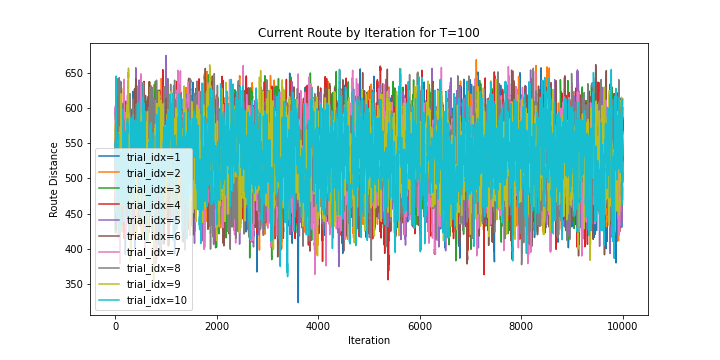
\includegraphics[scale=0.32]{figures/route_by_iteration_t=100_random.png}
      \caption{Searched Routes and Their Corresponding Tour Distance by Iteration for Different Temperature Values using Markov Chain Monte Carlo.}
      \label{fig:iteration_mcmc_2}
    \end{figure}

  \item It appears that generally speaking, the second approach of just selecting two random parks to swap tends to lead to discovering shorter tours. The reason for this is that the Markov Chain in (c) has a more distributed transition matrix, where each state has connections to $O(n^2)$ other states instead of just $O(n)$ as in (b). As such, the starting state is less important in this case, which further allows the system to mix faster. 

  This also explain why (c) requires a lower temperature. The easier mixing means that we need less randomess in order to avoid getting stuck in local minima. As such, we approach the stationary distribution much more quickly and easily. Too higher a temperature leads to suboptimal decisions.

\end{enumerate}

\newpage
\section*{Part 3}
\begin{enumerate}[label=(\alph*)]
  \item Does not need to be submitted.
  \item For the full code, please see the Appendix section. The input plan is given as per the below:
  \begin{verbatim}
  array([ 0.36,  0.49,  0.88,  0.85,  1.  ,  1.  ,  0.74,  1.  , -1.  ,
       -0.83,  0.29,  0.16,  0.8 ,  0.73,  0.57, -0.61,  0.77,  0.95,
       -0.96, -0.08, -0.3 , -1.  , -0.82, -1.  ,  0.95,  0.48, -1.  ,
        0.72, -0.78, -1.  , -0.11, -0.9 ,  0.78, -0.26,  0.57,  0.15,
        0.09, -0.88, -0.86, -0.5 ])
  \end{verbatim}

  A video of the above can be found here: https://youtu.be/kQFOffXiVMM
  \item We achieve a distance of 9.198867470630958. Our method is a simple modification of the MCMC method used in previous parts of the assignmet. We use $T = 0$ and define neighboring states as adding a uniform random value in the range $[-0.1, 0.1]$ (so changing the vector by at most $10\%$). Our local search implies that the nearby values are also good, as long as the inputs aren't changed too much. 

\end{enumerate}


\newpage
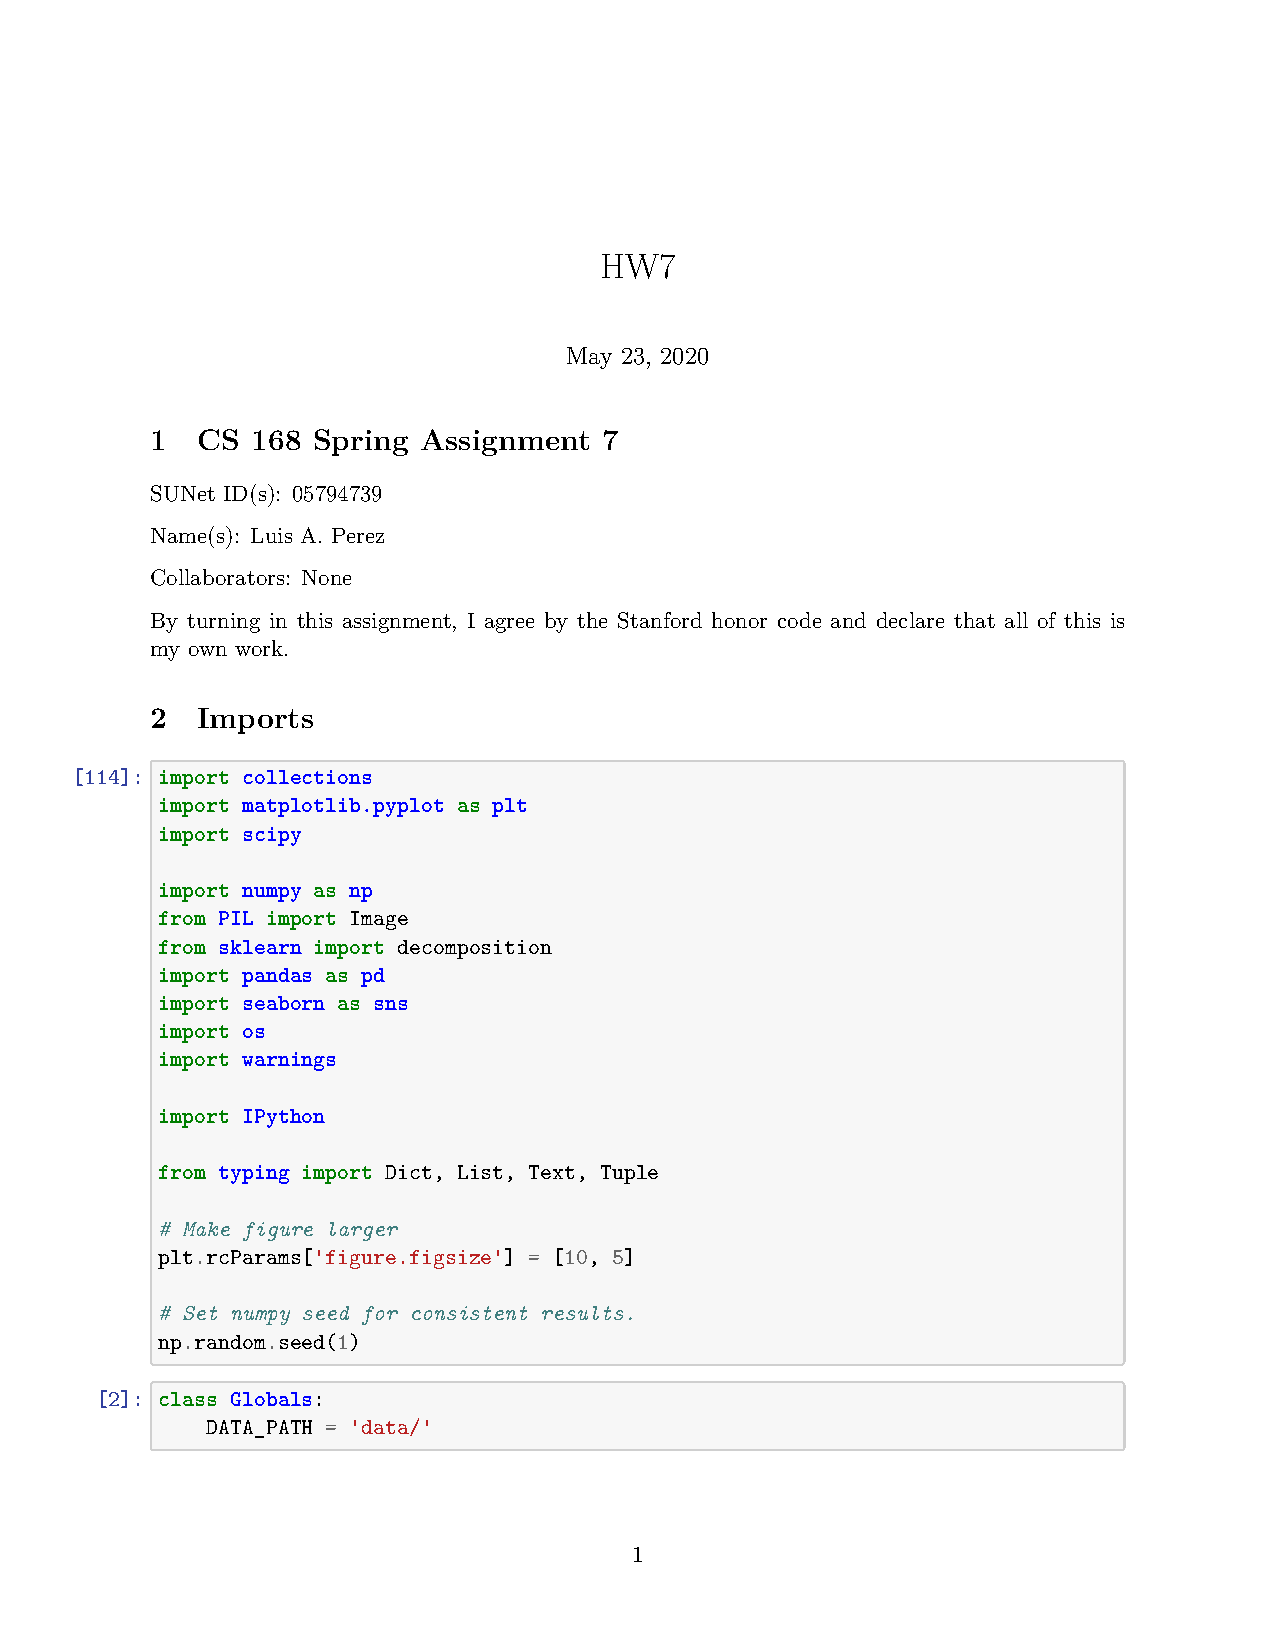
\includepdf[pages=-]{HW7}

\end{document}
